\chapter{Loosen control without losing control}
\label{multilevel:chapter}

In an interview for OpenSource.com in December 2015, Dries \parencite{losen-control:2016:Online} explained his views on how FLOSS communities manage to scale up while continuing to innovate:

\begin{figure}[H]
  \centering
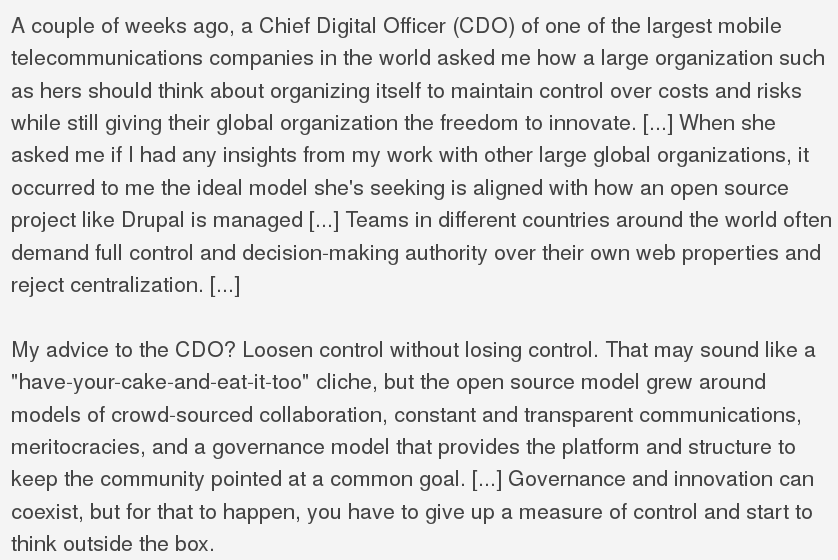
\includegraphics[width=\textwidth]{img/quotes_replacement/loosen_without_losing_controlS2.png}
\caption[Excerpt from the article ``How open source solves the innovation problem"]{Excerpt from the article ``How open source solves the innovation problem". Retrieved \nth{28} July 2016, from \url{https://opensource.com/open-organization/15/12/how-open-source-solves-innovation-problem}.}
\label{loosen_without_losing_control}
\end{figure}

This idea of ``loosen control without losing control" points precisely to the co-existence of these different forms of organisation in large CBPP communities, which, in the case of Drupal, materialised through the emergence of different socio-technical systems of contribution as explored in previous chapters.

On the one hand, the most formalised types of socio-technical systems ensure that activities requiring the highest levels of coordination, consistency and quality assurance are carried out. This was illustrated, for example, through the study of the organisational processes of the socio-technical system of development of \textit{core} projects or that of \textit{DrupalCons}. On the other hand, the simultaneous existence of more decentralised, autonomous and chaotic socio-technical systems is determinant as a force of disruption, experimentation and innovation. For example, this was illustrated by the case of the socio-technical system of \textit{custom} and \textit{contributed} projects, which resulted in the production of a notably rich but more fragmented set of digital commons, and
by that of local events and \textit{DrupalCamps}, which enable a transition of ideas and proposals.

This counterbalancing and complementary co-existence of socio-technical systems, in which different systems varying in degree of formality co-exist and interact with each other, is fundamental to understand, from a macro perspective, the resulting organisational configuration after the massive changes experienced by the Drupal community over time under continuous growth. Throughout the next sections, these organisational changes and the general dynamics identified in previous chapters are analysed drawing on several concepts from previous literature from diverse fields, such as design principles for successful self-governance, mechanistic and organic organisational structures and \textit{polycentric} governance.

Firstly, the overall changes experienced in the self-organisational processes of the Drupal community previously explored are explained on the basis of previous literature on CBPP, which drew on the principles for successful self-governance defined by \textcite[88-102]{ostrom1990governing} introduced in section \ref{subsec:governance-cbpp}. Despite these principles being originally derived from the study of self-organised communities managing natural resources, they remain valuable in providing ways to understand the reasons that led the Drupal community to carry out these changes, and allow previous studies of large and global CBPP communities such as Wikipedia to be drawn on.

Secondly, this analysis will draw on the concepts of organic and mechanistic organisational structures \parencite{burns1961management} to overcome some of the limitations from the aforementioned previous studies on large and global CBPP communities derived from Ostrom's principles. Drawing on these concepts, an analysis of the organisational characteristics of the socio-technical systems of contribution previously explored is presented, arguing that these characteristics are part of a more general organisational configuration affecting the whole of the Drupal community in which socio-technical systems with different degrees of \textit{organicity} co-exist and interact with each other.

Thirdly, this analysis will draw on the notion of \textit{polycentrism} in order to define the resulting governance model of the Drupal community which has emerged over time as part of the general dynamics of decentralisation and formalisation, resulting in a variant number of centres of authority. This notion also originates from studies of communities regulating more traditional commons, such as natural resources \parencite{ostrom1961organization}. \textit{Polycentric} ``connotes many centers of decision making that are formally independent of each other" \parencite[831]{ostrom1961organization}. The emergence of different socio-technical systems of contribution presented in previous chapters, it is argued, shows how Drupalistas have been able to organise themselves not just by one, but by multiple governing authorities at different levels of \textit{organicity}.

By bringing this literature together, the chapter concludes by tackling the main research question formulated in section \ref{subsubsec:state-art:drupal:case-study} ---  ``how does a large and global Commons-Based Peer Production community self-organise?" --- building a central argument which revolves around the emergence of a set of socio-technical systems varying in their degree of \textit{organicity} regulated by \textit{polycentric} governance.

\section{Drupal as a CBPP community}
\label{sec:ostrom}

Having framed this case study not only as a FLOSS community, as argued in section \ref{subsubsec:state-art:cbpp:commons:cbpp}, but as part of the phenomenon of CBPP, enables social theory to be called upon for the study of the Drupal community by exploring it as a distinct mode of production, an aspect missing in FLOSS studies as argued by \textcite{glaser2007social}. Thus, this section draws on previous literature on CBPP in order to contextualise and support the main argument presented throughout chapters \ref{sec:custom-to-contrib} to \ref{mostly-offline-cons:chapter}: the growth experienced by the Drupal community led to the formalisation of self-organisational processes facilitating decentralisation of decision-making in order for these processes to scale up. The dynamic of formalisation identified for this case study is congruent with the few previous qualitative studies \parencite{viegas2007hidden, forte2009decentralization} on the changes of self-organisational processes of other large and global CBPP communities which explored similar issues in Wikipedia. These previous studies also provide accounts of the emergence of formalised structures over time. Firstly, \textcite{viegas2007hidden}, questioned the predominant oversimplified depictions of self-organisation in Wikipedia's community at the time, in which self-organisation almost magically emerged in a chaotic space. They showed the existence of formal processes defined over time as the community grew. While the work of \textcite{viegas2007hidden} focussed on a single peer production process --- the selection of featured articles ---  the subsequent work by \textcite{forte2009decentralization} directly focussed on the governance of Wikipedia drawing on \textcite{viegas2007hidden}. In a similar way as in the case of the Drupal community, \textcite[71]{forte2009decentralization} concludes that the story of self-organisation in Wikipedia is that of increasing decentralisation, in which the community formalised processes as complexity grew over time. Both studies on Wikipedia draw on the principles defined by \textcite[88-102]{ostrom1990governing} for successful self-organisation introduced in section \ref{subsec:governance-cbpp} to explain the changes experienced in the self-organisational processes of the community. Despite these principles being originally derived from the study of self-organised communities managing natural resources, they also remain valuable in providing ways to understand the organisational changes identified for this case study. Table \ref{tab:ostrom} provides an overview of the main organisational changes explored throughout chapters \ref{sec:custom-to-contrib} to \ref{mostly-offline-cons:chapter} and their relationship with Ostrom's principles, following a similar approach as that carried out by \textcite{viegas2007hidden} and \textcite{forte2009decentralization} to explain the organisational changes experienced by another large and global CBPP community, Wikipedia.

\begin{footnotesize}
\begin{longtable}{|p{3cm}||p{4.7cm}|p{5.5cm}|}
\hline
Design principle & Related organisational changes in the Drupal community & Examples and references \\ \hline \hline
1. Clearly defined community boundaries
&
Emergence of clearer boundaries to participate in the production and management of projects and events.
&
Definition of core initiatives and gates (section \ref{subsec:dec-form-core}), boundaries for maintenance in \textit{contributed} projects (section \ref{subsec:emergence-contrib}), or specific membership for local (section \ref{subsec:dcamps-emergence-local-institutions}) and global institutions (section \ref{subsec:dec-form-modern-dcons}).
\\ \hline
2. Congruence between rules and local conditions
&
Emergence of autonomous spaces with regards to local decision-making in \textit{contributed} projects and local institutions to avoid a ``one-size-fits-all" regulation.
&
Local rules for projects in section \ref{subsec:emergence-contrib} or for local events, \textit{DrupalCamps} and local institutions (see chapter \ref{mostly-offline-local:chapter}).
\\ \hline
3. Collective-choice arrangements
&
Vast amount of collective-choice arrangements explored as part of a constant process to devise ways to increase participation in the elaboration of rules by those affected by them.
&
Rules for \textit{contributed} projects maintenance, (see section \ref{subsec:emergence-pap}), discussions related to the Core Gates (see section \ref{subsec:dec-form-core}), or rules regarding the management of institutions (see section \ref{subsec:dcamps-emergence-local-institutions}).
\\ \hline
4. Monitoring
&
Emergence of explicit roles and processes related to quality assurance so that certain individuals, accountable to the community, monitor the commons.
&
Monitoring via PAP (see section \ref{subsec:emergence-pap}) for \textit{contributed} projects, vast amount of roles for monitoring core (see section  \ref{subsec:dec-core-initiative}), or for the selection of presentations for \textit{DrupalCons} (see section \ref{subsec:dec-form-modern-dcons}).
 \\ \hline
5. Graduated sanctions
&
Development of codes of conduct.
&
Drupal, \textit{DrupalCon} and \textit{DrupalCamps} codes of conduct, enforced, for example, in banning attendance for tweeting derogatory comments about presenters ---  see section \ref{subsec:formalis-dcons}.
\\ \hline
6. Conflict resolution mechanisms
&
Definition of mechanisms to facilitate access to conflict resolution.
&
Definition of Drupal Community Working Group (see section \ref{subsec:dec-form-modern-dcons}).
\\ \hline
7. Local enforcement of local rules
&
Emergence of local jurisdiction and acknowledgement by the most centralised authorities of creation and enforcement of local rules. &
Local jurisdiction of \textit{contributed} projects (see section \ref{subsec:emergence-contrib}) with respect to Drupal core, or of local institutions (see Spanish Association in section \ref{subsec:dcamps-emergence-local-institutions}) with respect to the global institution.
\\ \hline
8. Multiple layers of nested enterprises
&
Overall emergence of socio-technical systems of contribution to address issues that affect the common resources differently at wider and local levels.
&
Emergence of socio-technical systems of \textit{core}, \textit{contributed} and \textit{custom} projects for the case of ``mostly-online" contribution activities; or \textit{DrupalCons}, \textit{DrupalCamps} and local events for ``mostly-offline" ones, presented throughout chapters \ref{sec:custom-to-contrib} to \ref{mostly-offline-cons:chapter}.
\\ \hline
\caption{Relationship between main organisational changes identified and Ostrom's principles.}
\label{tab:ostrom}
\end{longtable}
\end{footnotesize}

This connection between the study of organisational processes with the actions in their collective production processes \parencite{Mahony2011}, carried out in this study through the notion of contribution activity, contributes to the literature on FLOSS studies by providing a perspective which explored the phenomenon of FLOSS as a distinct mode of production \parencite{glaser2007social}, framing it not exclusively as a FLOSS community, but as a Commons-Based Peer Production community, and allows parallelisms to be found with the way self-organisation works in Wikipedia.

For example, the first of Ostrom's principles, which refers to the boundaries defined by the community to draw on the common resource, re-interpreted as the access to modify or organise in the context of digital commons by \textcite{forte2009decentralization}, aids the understanding of the reasons that led to an increase in formalisation in these communities. The organisational changes experienced by this case study resemble those of Wikipedia for peer production of articles: an overall trend towards a definition of clearer boundaries in the Drupal community was clearly identified for the socio-technical systems of contribution analysed, in this case in the form of commit permissions and their propagation to modify the source code. For example, as part of the changes related to Core Initiatives and Core Gates presented in section \ref{subsec:dec-form-core}, and by the emergence of delimited autonomous spaces presented in section \ref{subsec:emergence-contrib}, whose boundaries were reflected in the artefacts through the form of autonomous project pages.

Another example of Ostrom's principles which aids the understanding of the organisational changes experienced by the Drupal community is that related to the principle of acknowledgement of local jurisdiction to create and enforce the local rules by the most centralised authorities, as also shown for the case of Wikipedia. The findings from this study are congruent with those from the study of organisational processes carried out by \textcite{forte2009decentralization}, in which, as part of a similar general dynamic of decentralisation, they described the emergence of autonomous WikiProjects, whose jurisdiction to devise their own local rules is acknowledged by more central authorities. In the case of the Drupal community, however, these spaces have an even higher degree of autonomy than those described by \textcite[64]{forte2009decentralization} for Wikipedia.

Nevertheless, Ostrom's principles present limitations for the understanding of the resulting organisational structures which emerged in large and global CBPP communities, such as Drupal or Wikipedia, as a result of the aforementioned dynamics of decentralisation and formalisation. The overall emergence of the different socio-technical systems of contribution explored throughout chapters \ref{sec:custom-to-contrib} to \ref{mostly-offline-cons:chapter}, despite the focus of action being oriented towards a similar resource, such as source code or events, can only find a vague explanation when framed through Ostrom's general principles. The aforementioned studies on Wikipedia present similar limitations. The study by \textcite{viegas2007hidden} was limited by focusing on the changes in the organisational processes of a single peer-production process, whereas the emergence of WikiProjects as an illustration of the emergence of more decentralised and autonomous organisational structures was partially explained by \textcite{forte2009decentralization} through the last of Ostrom's principles. The authors, however, acknowledged these issues should be further explored \parencite[70-71]{forte2009decentralization}. Similarly, for the case of Drupal, since Ostrom's principles are aimed to be general and they were derived from the study of smaller communities, they are also vague when aiming to further understanding on the resulting counterbalancing and complementary co-existence of the socio-technical systems identified for this case study with more precision.

On the basis of these limitations, the subsequent section presents the results of an analysis carried out on the organisational characteristics of the previously explored socio-technical systems of contribution, drawing on classic literature from organisational theory with the aim to continue to shed light on the \textit{hidden order} \parencite{viegas2007hidden} of large and global CBPP communities, such as Drupal or Wikipedia.

\section{Degrees of \textit{organicity} in peer production}
\label{sec:levels-organicity}

This study began arguing for the need to further understanding of how self-organisation occurs in CBPP communities, beyond the current limitations present in the scarce CBPP literature in which it is stated that the underlying governance mechanisms differ from those of the ``market" or the ``firm" \parencite{Benkler2002}. Recalling the subsequent work of \textcite[61]{benkler2006wealth} in ``The Wealth of Networks", he stated that:

\begin{quotation}
``[...] the salient characteristic of commons, as opposed to property, is that no single person has exclusive control over the use and disposition of any particular resource in the commons. Instead, resources governed by commons may be used or disposed of by anyone among some (more or less well-defined) number of persons, under rules that may range from `anything goes' to quite crisply articulated formal rules that are effectively enforced."
\end{quotation}

Nevertheless, it was argued, there is a need for empirical studies which help to show how these rules emerge, are defined, enforced and evolve over time. Chapters \ref{sec:custom-to-contrib} to \ref{mostly-offline-cons:chapter} provide an in-depth account of these processes, which resulted in the emergence of new socio-technical systems of contribution for activities with a similar main focus of action (the development of source code or the organisation of events), and how these systems were shaped by dynamics of formalisation and decentralisation. Also discussed was the different degree of formalisation which the socio-technical systems of contribution have reached to the current day. Overall, the different characteristics and the simultaneous existence of all of these socio-technical systems around contribution activities exhaustively explored are not to be considered as isolated, but as part of a more general organisational configuration related to the self-organisation of the peer production activities of the Drupal community identified in section \ref{subsec:insights:contrib-beyond-source-code}. Nevertheless, although the degree of formalisation is a valuable indicator to identify and establish comparisons between these systems, it is insufficient for conceptualising all of the organisational characteristics identified in these socio-technical systems which emerged from the final stage of the analysis carried out in this study. The classic concepts from organisational theory of organic and mechanistic organisational structures \parencite{burns1961management} provide a more accurate way to capture the richness of the organisational characteristics of these socio-technical systems of contribution, since these concepts better subsume the characteristics which emerged from the general analysis, including the degree of formalisation.

On the one hand, mechanistic structures are characterised by higher degrees of formalisation and centralisation. The hierarchies are more explicit and well-defined and the decision-making follows a top-down approach. They also involve higher degrees of specialisation and an explicit division of labour. Processes are bureaucratic, rigid and more resistant to change. On the other hand, organic organisational structures have higher degrees of informality and decentralisation. They lack rigid procedures and involve lower levels of specialisation. The division of labour is blurred, if existent, and decision-making is based on the needs felt by the participants, presenting similarities with that subsumed by the concept of ``do-ocracy" employed by studies on hacker culture. Organic structures represent the most adaptive forms of organisation, in which changes can be quickly implemented according to varying contexts.

Rather than binary, in the Drupal community, \textit{organicity} and \textit{mechanisticity} are better thought of as part of a spectrum in which the organisational structures of the community lie. This is in line with previous studies on organisation \parencite{harrison1972professional, bahrami1987stratocracy, louadi1998relationship, green2008exploring, ireland2009conceptualizing, chelliah2010determinants, mallen2016organicity} which defined a degree of structural \textit{organicity}. Developing from this concept of degree of \textit{organicity}, the overall analysis carried out of the main organisational characteristics of the socio-technical systems of contribution revealed the co-existence of three different categories according to the degree of \textit{organicity} of the peer production processes of this case study: high, intermediate and low. The results of this analysis show the simultaneous existence of organisational forms with different degrees of \textit{organicity} in large and global Commons-Based Peer Production communities. As in the case of the general dynamics presented in previous chapters, the findings suggest these categories transcend the online/offline dimension, despite the inherent differences resulting from the main medium by which the activities are carried out. Table \ref{tab:layers-summary} provides an overview of the main characteristics which emerged from the final stage of the analysis for each of these categories:

\begin{footnotesize}

\begin{longtable}{|p{3cm}||p{3.4cm}|p{3.4cm}|p{3.4cm}|}
\hline \hline
\def\arraystrecth{1.5}
\multirow{2}{3cm}[\normalbaselineskip]{Characteristics of organisational processes} & \multicolumn{3}{c|}{Degree of \textit{organicity}} \\ \cline{2-4}
\strut & \textsl{d\textunderscript{1}}: High & \textsl{d\textunderscript{2}}:  Intermediate & \textsl{d\textunderscript{3}}: Low \\ \hline \hline \hline
\def\arraystrecth{1}

Amount of explicit rules &
Based on implicit rules. For example, `writing good code' or `avoiding promotional talks' (see section \ref{subsec:local-events}). &
Intermediate amount of rules partially affecting areas (e.g. quality assurance). For example, coding standards (see section \ref{subsec:emergence-pap}) or selection criteria for presentations (see section \ref{subsec:dcamps-dtd}). &
Large amount of explicit rules affecting most areas, such as governance, quality assurance and division of labour. For example, Core Gates (see section \ref{subsec:dec-form-core}) or conflict of interest regulation (see section \ref{subsec:dcons-growth}). \\ \hline

Specialisation &
Implicit and blurred division of labour. For example, attendee or presenter (see section \ref{subsec:local-events}). &
Intermediate levels of division of labour, explicit in some cases. For example, maintainers of \textit{contributed} projects (see section \ref{subsec:emergence-pap}), or organisers of \textit{DrupalCamps} (see section \ref{subsec:dcamps-dtd}). &
Explicit and large division of labour. High degree of specialisation. For example, product owners, core committers, release managers and track chairs (see sections \ref{subsec:dec-form-core} and \ref{subsec:dec-form-modern-dcons}). \\ \hline

Degree of formality &
Low degree of formality. For example, social life organised around implicit social rules (see section \ref{subsec:local-events}) and not requiring formal organisational structures (see section \ref{subsec:emergence-contrib}). &
Intermediate degree of formality. Emergence of some formal organisational structures (see section \ref{subsec:emergence-pap}) and local institutions, such as the Spanish Drupal Association (see section \ref{subsec:dcamps-emergence-local-institutions}). &
High degree of formality. Organised around the most formal organisational structures and institutions, with bureaucratic processes for most of the decision-making. For example, the development of core (see section \ref{subsec:dec-form-core}) and the Drupal Association (see section \ref{subsec:dec-form-modern-dcons}). \\ \hline

Centralisation and autonomy &
Fully decentralised spaces and loosely interconnected: vast amount of small centres of decision-making almost completely independent of each other (see section \ref{subsec:local-events}). &
Considerable amount of medium-sized autonomous distributed spaces with low degrees of dependence on others. For example, \textit{contributed} projects working groups (see section \ref{subsec:contrib-day-by-day}), or the Spanish Drupal Association (see section \ref{subsec:dcamps-emergence-local-institutions}). &
The most centralised and rigid structures, several centres of decision-making with stronger interdependence between them. For example, the Core Governance (see section \ref{subsec:dec-form-core}) or committees in the Drupal Association (see section \ref{subsec:dec-form-modern-dcons}). \\ \hline

Complexity and amount of required coordination &
Low degree of required coordination in the activity and low levels of complexity of main focus of action (see sections \ref{subsec:emergence-contrib} and \ref{subsec:local-events}). &
Intermediate degree of required coordination and complexity of main focus of action, for example \textit{contributed} projects (see section \ref{subsec:emergence-pap}) and \textit{DrupalCamps} (see section \ref{sec:growth-community}). &
Largest amounts of required coordination and main focus of action highly complex. For example, Drupal core and \textit{DrupalCons} (see section \ref{sec:growth-community}).  \\ \hline

Legitimacy &
Low level of legitimacy in the community required to organise activities. For example, to create a project not within the main collaboration platform (see section \ref{subsec:emergence-contrib}) or do a call for a local event (see section \ref{subsec:local-events}). &
Intermediate level of legitimacy to organise activities. For example, to develop a \textit{contributed} project (see section \ref{subsec:emergence-pap}) or to organise a \textit{DrupalCamp} (see section \ref{subsec:dcamps-emergence-local-institutions}). &
Requiring a high level of legitimacy in the community. For example, to run a core initiative (see section \ref{subsec:dec-form-core}) or to organise a \textit{DrupalCon} (see section \ref{subsec:dec-form-modern-dcons}). \\ \hline

Perceived value of contribution activities  &
Perceived as less valuable by members of the community and providing lower levels of gained reputation to contributors. For example, publishing a project not within the main collaboration platform (see section \ref{subsec:emergence-contrib}) or to speak at a local event (see section \ref{subsec:local-events}). &
Intermediately valued by the members of the community and providing intermediate levels of gained reputation to contributors. For example, maintaining a \textit{contributed} project (see section \ref{subsec:contrib-day-by-day}) or speaking at a \textit{DrupalCamp} (see section \ref{subsec:dcamps-emergence-local-institutions}). &
Highly valued by the members of the community and providing high levels of gained reputation to contributors. For example, maintaining a \textit{core} project (see section \ref{subsec:insights:contrib-beyond-source-code}) or speaking at a \textit{DrupalCon} (see section \ref{subsec:dcons-day-to-day}).  \\ \hline

Ease/difficulty to participate or modify commons. &
Easy to participate, organise or modify. For example, to publish a project not within the main collaboration platform (see section \ref{subsec:emergence-contrib}) or to be selected to speak at a local event (see section \ref{subsec:local-events}). &
Intermediate level of ease to participate. For example, to publish a \textit{contributed} project (see section \ref{subsec:emergence-pap}) or to be selected to speak at a \textit{DrupalCamp} (see section \ref{subsec:dcamps-emergence-local-institutions}). &
Highest barriers to participate. For example, to run a \textit{core} initiative (see section \ref{subsec:dec-form-core}) or to be selected to speak at a \textit{DrupalCon} (see section \ref{subsec:dcons-day-to-day}).  \\ \hline

Required Quality Assurance &
No communitarian quality assurance mechanisms, for example of projects not within the main collaboration platform (see section \ref{subsec:emergence-contrib}); or extremely basic if any, for example discarding promotional sessions in local events (see section \ref{subsec:local-events}). &
Intermediate level of quality assurance with explicit mechanisms in some areas. For example, the PAP process for \textit{contributed} projects (see section \ref{subsec:emergence-pap}) or the selection of presentations by organisers in \textit{DrupalCamps} (see section \ref{subsec:dcamps-emergence-local-institutions}). &
High levels of quality assurance. Explicit mechanisms and processes affecting most areas. For example, Core Gates (see section \ref{subsec:dec-form-core}) or rules to designate selectors and conflict of interest regulation in \textit{DrupalCons} (see section \ref{subsec:dcons-growth}). \\ \hline

Degree of required consistency of main focus of action &
Extremely fragmented. No need for consistency. Independent from other initiatives at the same level. For example, lower level of interdependency of projects not within the main collaboration platform (see section \ref{subsec:emergence-contrib}) or between local events even in the same area (see section \ref{subsec:local-events}). &
Intermediate levels of required consistency. Partial interdependence with other initiatives at the same level. For example, interdependency between some \textit{contributed} projects and processes to avoid fragmentation (see section \ref{subsec:emergence-pap}), or between holding \textit{DrupalCamps} in the same region or country (see section \ref{subsec:dcamps-emergence-local-institutions}). &
High need for consistency in the main focus of action. For example, strong interdependency between all \textit{core} projects (see section \ref{subsec:dec-form-core}), or critical consistency on holding \textit{DrupalCons} (see section \ref{subsec:dcons-growth}). \\ \hline

\caption[Summary of main characteristics of categories according to different degrees of \textit{organicity} identified in the organisational processes of the Drupal community.]{Summary of main characteristics of categories according to different degrees of \textit{organicity} identified in the organisational processes of the Drupal community.}
\label{tab:layers-summary}
\end{longtable}
\end{footnotesize}

Firstly, the existence of systems with the highest degrees of \textit{organicity} (\textsl{d\textunderscript{1}}), is illustrated by the socio-technical systems composed of local events and \textit{custom} projects, not within Drupal.org. In these socio-technical systems, the commons can be easily organised or created, duplicated or even forked. For example, calling for a local event or publishing a \textit{custom} project is a highly straightforward process which does not require significant legitimacy in the eyes of the community. Some of the main organisational characteristics for the most organic systems are their high degree of decentralisation, the ease with which it is possible to participate, and they remain less affected by the dynamic of formalisation overall. However, these socio-technical systems are also the most chaotic and fragmented, and their resilience resides exactly in this distributed and more organic nature. Contributions to them are also typically perceived as less valuable according to the internal logics of value of the community and, as a consequence, contribution provides lower gains in reputation to the actors involved in them.

Secondly, \textit{DrupalCamps}, for ``mostly-offline",  and \textit{contributed} projects, for ``mostly-online", illustrate the existence of socio-technical systems with an intermediate degree of \textit{organicity} (\textsl{d\textunderscript{2}}). These systems require higher degrees of coordination and quality control than those that are more organic. As a consequence, they are more greatly influenced by the general dynamic of formalisation than those of \textsl{d\textunderscript{1}} resulting, for example, in the definition of clearer boundaries for participating in their modification or organisation as a commons. At the same time, this dynamic of formalisation allows them to scale up over time via the decentralisation of decision-making, while increasing the legitimacy, in the eyes of the community, of actors and institutions involved in them. Overall, socio-technical systems presenting this intermediate degree of \textit{organicity} represent the emergence of numerous, distributed and autonomous spaces, which are a source of constant innovation and experimentation.

Thirdly, \textit{DrupalCons} and \textit{core} projects illustrate the existence of socio-technical systems with the least organic, or the most mechanistic, characteristics (\textsl{d\textunderscript{3}}). The commons at this level require the highest levels of consistency, quality assurance and coordination. For example, in the case of ``mostly-online" activities this was reflected in the need for greater quality assurance and consistency for source code; while in the case of ``mostly-offline", it was reflected in the need for consistency in the organisation of events, and high levels of quality assurance with respect to the activities carried out, such as the selection of presentations. As presented in chapter \ref{identifyng-contribution:chapter}, these are also contribution activities commonly perceived as more valuable according to the internal logics of value in the community and, thus, provide a greater reputation to the actors involved in them. For example, as a speaker at Drupal events, presenting at a \textit{DrupalCon} is perceived as adding to reputation more than at a \textit{DrupalCamp}, and similarly presenting at a \textit{DrupalCamp} is perceived as adding to reputation more than at a local event.

The characteristics of organisational processes for the different categories which emerged from the analysis, summarised in table \ref{tab:layers-summary}, are to be interpreted as interrelated, rather than isolated. An example of this interrelationship is that between the amount of explicit rules, division of labour and quality assurance required at different levels. Socio-technical systems of contribution activities presenting the most mechanistic characteristics (\textsl{d\textunderscript{3}}), whose main focus of action requires the highest levels of quality assurance, have a high degree of specialisation with explicit rules including for the division of labour. For instance, recalling the selection of presentations for \textit{DrupalCons}, explicit rules are defined for the selection of the selectors with the explicit figures of global and local track chairs to ensure a high degree of quality assurance --- see section \ref{subsec:dcons-day-to-day}. For those with an intermediate degree of \textit{organicity} (\textsl{d\textunderscript{2}}), the selection might commonly be carried out by the whole group of organisers, who are informally self-elected, and explicit rules for selectors do not commonly exist (see section \ref{subsec:dcamps-dtd}). However, there are explicit rules regarding the criteria for the selection of presentations, and, therefore, a high degree of quality assurance, although rules are not as exhaustive as for systems at \textsl{d\textunderscript{3}}. For the most organic (\textsl{d\textunderscript{1}}), there are not even explicit rules for these selection criteria, and the process is wholly based on informal mechanisms of control (e.g. through social norms) --- see section \ref{subsec:local-events}.

Another example of the interrelationship between these characteristics according to the degree of \textit{organicity} is that between perceived value, quality assurance and the degree of required consistency of the main object and its complexity. For instance, as presented in chapter \ref{chapter:core-system}, the organisational processes of \textit{core} projects (\textsl{d\textunderscript{3}}) require the highest degree of consistency. There are many dependencies in the object, the core, and a change in the code will affect all of the installations of Drupal websites in the World. Hence, the acceptance of a patch modifying even a single line of code is subject to the most strict and careful quality assurance processes defined in the community. As noted in chapter \ref{identifyng-contribution:chapter}, having a patch committed to core is perceived as a highly valued contribution, and a sign of a greater reputation. On the contrary, a commit in a module hosted outside of Drupal.org (\textsl{d\textunderscript{1}}), for example hosted in GitHub, does not require such consistency. Neither are there quality assurance processes regulated by the community. As shown in section \ref{subsec:emergence-contrib}, these contributions are perceived as hardly valuable, if at all, and they are not reflected in the main artefacts of collaboration --- see section \ref{subsec:insights:representation}. On the other hand, having a patch committed to a \textit{contributed} project (\textsl{d\textunderscript{2}}) requires intermediate levels of quality assurance, which are enforced by the maintainers of that project. The perceived value depends on the complexity, popularity and required degree of consistency of the project among other factors. For example, having a commit in a popular module, on which many other \textit{contributed} projects and Drupal sites depend, requiring a higher degree of consistency, is perceived as a more valuable contribution than having a commit in a lesser known \textit{contributed} project which is still in a sandbox status --- see section \ref{subsec:emergence-pap}.


Activities within these systems with different degrees of \textit{organicity} are not to be thought of as existing in isolation, but interacting and influencing each other as part of the networks of socio-technical systems of contribution which they form. As part of this final stage of the analysis, a study of the interactions between these different socio-technical systems of contribution was also carried out. This analysis drew on the concept of interactions between several activity systems from the third generation of Activity Theory (see section \ref{subsec:3at}), with the aim of furthering understanding of the dynamism of the resulting co-existing organisational forms \parencite[34]{kuutti1996activity}:

\begin{quotation}
``[...] activities are not isolated units but are more like nodes in crossing hierarchies and networks, they are influenced by other activities and other changes in their environment. External influences change some elements of activities, causing imbalances between them. [...]"
\end{quotation}

This analysis\footnote{These interactions emerged from an overall analysis drawing on the concept of tension from Activity Theory, presented in chapter \ref{sec:theoretical-frameworks}. Interactions between activity systems were subsumed as part of the overall identification of tensions which emerged from the collected data (see appendix \ref{appendix-list-conflicts}). Unsurprisingly, these identified tensions cover a wide range of topics affecting all relevant entities from an Activity Theory perspective. It is clear that not all of these tensions are interpreted by Drupalistas as having a positive effect in the long term for the sustainability of the community. For example, the creation of a fork of Drupal's core (see section \ref{subsec:d7-d8}) can be interpreted as a result of a tension due to the disagreement of some Drupalistas with the direction the project took in the transition from Drupal 7 to Drupal 8, which caused a fear of a possible division of the community.} revealed how socio-technical systems of contribution with a similar main focus of action (e.g. a project or an event) but with different degrees of \textit{organicity} interact and influence each other. This influence occurs in both directions: from mechanistic to organic and vice versa. 

For the first direction, an extension of practices from mechanistic systems increasing the degree of formalisation of more organic systems  emerged as the clearest example of influence. An illustrative example of these interactions for the case of ``mostly-online" activities refers to the practice of using automated testing\footnote{Automated tests are separated pieces of source code intended to test certain functionalities by comparing the outcomes with a set of predicted ones.}, which was defined as a compulsory and explicit policy in order to accept contributions \parencite{drupal8-automated-tests:2016:Online}, also generating tensions in the \textit{contributed} socio-technical system. Drupalistas managing \textit{contributed} projects had to tackle questions such as: should this policy be mandatory for their \textit{contributed} projects? Will this create more barriers for possible contributors? While a global mandatory policy was never implemented, in line with Ostrom's principle of ``congruence between rules and local conditions", it was observed how this practice has been adopted in the development of certain \textit{contributed} projects, more commonly those presenting the highest levels of activity and contributors. Similar extensions of practices from mechanistic to intermediate or the most organic socio-technical systems were also found for the case of ``mostly-offline" contribution activities, showing, for example, a wide extension of practices regarding the governance of regional or national institutions inspired by those of the Drupal Association. An illustrative example of this concerns the development and use of Codes of Conduct, such as those discussed in section \ref{subsec:dec-form-modern-dcons}. For example, the definition of the \textit{DrupalCon} Code of Conduct, aiming to comprise the shared values of the Drupal community in order to create a safe and welcoming environment in these events, also generated tensions in more organic systems related to the organisation of events. In this case, local communities had to face questions such as: should the \textit{DrupalCon} or Drupal Codes of Conduct, or variations, be adopted in our \textit{DrupalCamp}? What would be the consequences of adopting it? Are these events also becoming ``too formal and bureaucratic"? As in the case of \textit{contributed} projects, the jurisdiction resides with the autonomous groups which organise the \textit{DrupalCamp} and, analogously, its use is not compulsory globally, but the practice of using the \textit{DrupalCon} or Drupal Codes of Conduct, or variations of them, in \textit{DrupalCamps} was extended to many of these events\footnote{See, for instance, \url{http://drupalcampnorth.org/code-of-conduct} and \url{http://2016.fldrupal.camp/community/code-conduct/index.html} for examples of the use of codes of conduct for \textit{DrupalCamps} in a European and a US \textit{DrupalCamp} respectively (retrieved \nth{20} September 2016).}. Overall, this can be interpreted as interactions in a similar way as those from ``mostly-online" activities: a practice increasing the degree of formalisation in the most mechanistic socio-technical system, generating tensions in more organic systems, which may result in an extension of practices.

Interactions were also identified in the reverse direction: the collected data showed the influence of more organic systems on more mechanistic systems as a source of change and disruption. For example, for ``mostly-online" activities, \textit{contributed} projects emerged as \textit{arenas} for experimentation and innovation, in which certain projects may eventually become part of core and, hence, influence to the point of changing the general technical direction of the project\footnote{As previously depicted by graph \ref{core-modules-release}, the number of projects in each new version of Drupal has been almost constantly growing, and these new projects are commonly \textit{contributed} ones transitioning to become core. The diff version of the automatically generated list of projects in core at \url{https://www.drupal.org/node/1283408/revisions} illustrates these transitions from September 2011. The initial stages of the case study of the ``Twig in Core" initiative presented in section \ref{subsec:dec-core-initiative} are an example of these transitions of projects, in which the initial ideas and initiatives were experimented and developed in more organic systems --- such as the examples of the \textit{Mothership} and \textit{Style Stripper} projects discussed in subsection \ref{subsec:themers-itch} --- and ended up being part of core. The case of \textit{Views}, a highly popular project in the Drupal community disrupting the main direction of the project represents another illustrative example, whose inclusion in Drupal 8 was defined as a ``cry out of the community" by many Drupalistas when the topic was discussed during observation.}. For the case of ``mostly-offline" contribution activities, organic socio-technical systems emerged as analogous \textit{arenas} to present and discuss ideas, proposals and critiques in the community, which can eventually be exposed in major scenarios, such as presentations in \textit{DrupalCons}, where these ideas increase their possibility of impact. These trajectories of ideas and proposals from organic towards mechanistic systems in the form of presentations resemble those of projects: more organic systems are sources of change and disruption. For example, as part of my participant observation with the community, I could observe this type of influence through a series of presentations of my own ideas to the community of the findings discussed in chapter \ref{identifyng-contribution:chapter}. I started presenting them at a local event \parencite{talk-silver-show-tell:Online}, at a later stage I presented as a keynote speaker at a \textit{DrupalCamp} \parencite{talk-silver-dcnorth:Online}, and finally as part of a community keynote celebrated at a \textit{DrupalCon} \parencite{talk-silver-dconbcn:Online}. This fostered a discussion \parencite{impact-contrib01:Online, impact-contrib02:Online, impact-contrib03:Online, impact-contrib04:Online, impact-contrib05:Online, impact-contrib06:Online, impact-contrib07:Online, impact-contrib08:Online, impact-contrib10:Online} about the notion of contribution in the community and the need to make visible and acknowledge ``community-oriented" contribution activities, also affecting the most mechanistic systems. The community is tackling questions such as: ``How can we \textit{give weight} to the value of them? How can we track ``community-oriented" contributions?

Overall, the study of the emergence, definition, enforcement and changes over time of the procedural side of a large and global CBPP community presented in this thesis, provides empirical evidence of the emergence of co-existing forms of organisation in CBPP communities varying in their degree of \textit{organicity} and influencing each other. These findings further our understanding of self-organisation in peer production with respect to the scarce literature on CBPP, thus, improving our knowledge of the \textit{hidden order}, in the words of \textcite{viegas2007hidden}, of large and global CBPP communities, beyond the idea of CBPP communities having ``rules that may range from `anything goes' to quite crisply articulated formal rules" \parencite[61]{benkler2006wealth}.

In sum, the aforementioned dynamics of formalisation and decentralisation identified for this large and global CBPP community resulted in the emergence of several co-existing socio-technical systems of contribution with different degrees of \textit{organicity} resembling similar structural characteristics, despite the significant differences between the types of activities, for example in their main focus of action (creating code or organising events) or main medium (online/offline).

\section{The emergence of \textit{polycentric} governance in peer production}
\label{sec:hybrid-poly}

Having provided empirical evidence of the emergence of co-existing organisational forms varying in their degree of \textit{organicity} for this case study, a last question then arises: what kind of governance model, regulating these organisational processes, emerged in the Drupal community as a result of the aforementioned dynamics of formalisation and decentralisation? As discussed in section \ref{sec:do-ocracy}, Drupalistas, including Dries himself, indicate that the community is organised through a ``do-ocratic" model of governance \parencite[e.g.][]{do-ocracy01:2016:Online, do-ocracy02:2016:Online, do-ocracy03:2016:Online, do-ocracy04:2016:Online, do-ocracy05:2016:Online}. The characteristics of a ``do-ocratic" model described by Drupalistas resemble those of the bazaar governance \parencite{Demil2006} of FLOSS studies, examined in section \ref{floss-governance}, which was subsequently criticised \parencite{mateos2008institutions} for drawing on a simplistic full-egalitarian assumption, calling for the exploration of the emergence of the rules, norms and standards in FLOSS communities, as that carried out in this study, in order to shed light on how participation is regulated.

Thus, as previously argued in section \ref{sec:do-ocracy}, neither ``do-ocracy" nor bazaar governance capture the complexity of the governance model of the Drupal community after the massive organisational changes previously explored. While, as shown, the concept is useful to understand governance during the initial stages, the types of structures which emerged over time, especially the most mechanistic, differ radically from it. Instead, ``do-ocracy" should be understood as a set of shared values in the Drupal community, which has been determinant in shaping the ways in which the governance model evolved over the years, as shown throughout the previous chapters.

The general dynamics of decentralisation and formalisation and the emergence of the socio-technical systems presented in chapters \ref{sec:custom-to-contrib} to \ref{mostly-offline-cons:chapter} show, however, that the increasing need for coordination throughout the continuous growth of the community resulted in the emergence of a varying number of centres of authority, and that these centres vary in their degree of \textit{organicity}, as shown in section \ref{sec:levels-organicity}. When analysed from a macro perspective, the organisational changes presented in previous chapters illustrate the overall emergence of these multiple governing authorities for the regulation of the organisational processes of some of the most relevant contribution activities in the life of the community. In other words, these changes show how hundreds of thousands of Drupalistas have been able to organise themselves not just by one, but by multiple governing authorities at different levels of \textit{organicity}, as a result of the growth experienced by a community which originated from a small FLOSS project by a Belgian student in 2001 to become one of the most visible examples of Commons-Based Peer Production.

Rather than a ``do-ocracy", this study concludes that the development of these multiple governing authorities as a result of the identified dynamics of formalisation and decentralisation in the Drupal community represents the emergence of \textit{polycentric} governance. The notion of \textit{polycentrism} from which this study develops is that of \textcite*{ostrom1961organization} employed in the study of communities regulating commons such as natural resources \parencite[e.g.][]{gelcich2014towards}, which refers to the co-existence of several centres of governance which blend the distribution of authority and power with effective coordination between these centres. Although originally coined for the study of the organisation of government in metropolitan areas, and subsequently employed for the study of self-governance of natural resources, the concept of \textit{polycentric} governance has been more recently employed to further understanding of self-governance in communities managing the peer production of digital commons, such as Wikipedia \parencite{hartswood2014towards}.

In the case of ``mostly-online" activities, for example, the \textit{polycentric} character of the governance model of the Drupal community is illustrated by the emergence of autonomous spaces for decision-making on how to regulate the maintenance of \textit{contributed} projects examined in chapter \ref{sec:custom-to-contrib}, or by the definition of the working groups in core presented in section \ref{subsec:dec-form-core}. Similarly, for the case of ``mostly-offline" activities, it is shown by the emergence of numerous autonomous local groups and institutions holding events of different scopes explored in chapters \ref{mostly-offline-local:chapter} and \ref{mostly-offline-cons:chapter}.

In the end, the story told through the exploration of organisational changes in previous chapters is that of continuous negotiation, emergence and development of organisational structures to constantly seek to distribute authority in order to scale up decision-making, in which the participants in peer production systems  ``have authority to make at least some of the rules related to the use of that particular resource" \parencite[528]{ostrom1999coping}. This constant negotiation was illustrated, for example, by the emergence, definition and enforcement of the rules regarding the quality assurance processes of the activities previously examined. For instance, in the case of ``mostly-online" activities,  this was illustrated by the Project Application Process (PAP) of \textit{contributed} projects presented in section \ref{subsec:emergence-pap}, or by the Core Gates and Initiatives discussed in section \ref{subsec:dec-form-core}. Analogously, for the case of ``mostly-offline" activities, it was depicted by the processes related to the definition of quality assurance for the selection of presentations at \textit{DrupalCamps} explored in the case study in section \ref{subsec:dcamps-emergence-local-institutions}, as well as those related to the selection criteria for presentations and selectors of \textit{DrupalCons} examined through the case study in section \ref{subsec:dec-form-modern-dcons}. Overall, these processes illustrate how the autonomy and legitimacy to define rules in these different spaces emerged and how authority was distributed and legitimised over time.

While the ontological use of the concept of \textit{polycentricity} \parencite[13-15]{thiel2016polycentricity} enables light to be shed on the understanding of the governance of complex, adaptive socio-technical systems, such as those which emerged in the Drupal community, \textit{polycentric} governance as an explanatory theory has tended, however, to emphasise structuralist and static perspectives \parencite[8-9]{thiel2016polycentricity}. In other words, when \textit{polycentric} governance has been used as an analytical lens, these explanations have favoured approaches which assume stability, rather than dynamism and change, resulting in a lack of studies on  ``how it [\textit{polycentricity}] emerged, sustains or outlives itself" \parencite[7]{thiel2016polycentricity}.

In this way, the explored changes in the organisational processes and the identified dynamics of decentralisation and formalisation, in chapters \ref{sec:custom-to-contrib} to \ref{mostly-offline-cons:chapter}, as well as the interactions between socio-technical systems of contribution, as those discussed in section \ref{sec:levels-organicity}, contribute to the literature by providing a dynamic approach of how such a \textit{polycentric} model of governance has emerged in a large and global Commons-Based Peer Production community, while also shedding light on how participation is regulated in FLOSS communities beyond the model of bazaar governance \parencite{Demil2006}.

\section{Conclusion}

This chapter provided an analysis which brought together the study of socio-technical systems of contribution, presented in previous chapters, with literature related to the study of macro organisational aspects, in order to tackle the main research question. Thus, returning to the research question which has driven this study, ``how does a large and global Commons-Based Peer Production community self-organise?", this study concludes that, on the basis of the emergence of the socio-technical systems of contribution and the organisational changes explored and analysed throughout the previous chapters, the story of how the Drupal community self-organises is that of the emergence of an organisational system for peer production characterised by the counterbalancing and simultaneous co-existence of socio-technical systems of contribution varying in their degree of \textit{organicity}, in which Drupalistas have developed multiple governing authorities. Systemic contradictions, tensions and interactions between socio-technical systems have shaped, and continue to shape, an organisational system for peer production regulated by \textit{polycentric} governance on the basis of continuous negotiation amongst the participants.

In sum, this study furthers our understanding of the phenomenon of CBPP by providing an in-depth account of the organisational changes, which were shaped by a series of identified dynamics of formalisation and decentralisation, experienced by a community which originated from a small amateur FLOSS project by a student and was joined by hundreds of thousands of participants over the past fifteen years, showing how Drupalistas distributed authority and power over several centres of governance with effective coordination amongst them.

In order to build this argument, this chapter brought together literature from general theories of self-organising communities, organisational theory and empirical studies of other CBPP communities, in order to  connect the exploration of socio-technical systems of contribution with macro organisational aspects. Firstly, the overall changes in the self-organisational processes previously explored for this case study were explained drawing on previous literature on CBPP, an aspect missing in FLOSS studies. This thesis, it was argued, links the study of organisational processes with the actions in collective production processes through the notion of contribution, providing an approach which explored FLOSS as part of a distinct mode of production. While this literature supports the argument for the existence of intertwined dynamics of formalisation and decentralisation of decision-making experienced by the Drupal community and connect it to the phenomenon of CBPP, it was also argued that these general theories present limitations with regards to the resulting varying set of co-existing organisational structures identified in the community. For this reason, an analysis of the main organisational characteristics of the socio-technical systems previously explored was presented, drawing on the concepts of organic and mechanistic organisational structures from organisation studies. The dynamics of formalisation and decentralisation identified for this case study resulted in the emergence of several co-existing forms of organisation characterised for their different degrees of \textit{organicity}, despite the significant differences between the types of activities studied: developing source code and organising events. These general organisational characteristics identified from this case study, it was argued, further our understanding of self-organisation in large and global CBPP communities.

Having identified this simultaneous co-existence of organic and mechanistic organisational structures, the chapter finally focussed on how these different organisational forms are regulated, arguing that the organisational changes explored, as shaped by the dynamics of formalisation and decentralisation, illustrate the overall emergence of a \textit{polycentric} model of governance regulating these peer production processes. Having provided this in-depth account of the changes experienced in the organisational processes and the general dynamics which resulted in \textit{polycentric} governance, this study is novel in providing an approach which highlights dynamism and change in self-organisation, contrasting with the assumption of stability found in previous studies drawing on the same concept of \textit{polycentricity}.

This chapter concludes the presentation of findings and analysis which have formed the main body of this thesis, whose main contributions will be summarised in the next, and final, chapter.